\section{\bfseries Opis baze podataka}
%slika
Baza je predstavljena dijagramom klasa na slici \ref{fig:ClassDiagramDatabase}

U bazi su opisane tri grupe podataka:
\begin{itemize}
% izmenite slobodno nazive ovih grupa ako vam se ne svidjaju
    \item podaci o zaposlenima i snabdevačima
    \item podaci o klijentu i porudžbinama
    \item podaci o namirnicama i dostavi
\end{itemize}

\subsection{Podaci o zaposlenima i snabdevačima}
\subsection{Podaci o klijentu i porudžbinama}

\textbf{\large Klijent}
\vspace{0.3cm}

Klasa \textit{Klijent} predstavlja jednog klijenta, njegove lične podatke kao i preference oko plana ishrane.

Atributi:
\begin{itemize}
    \item id - jedinstveni identifikator klijenta (PK, automatski generisan)
    \item korisničkoIme 
    \item lozinka
    \item mejl
    \item brojPlatneKartice
    \item statusPretplate
    \item adresaDostave
    \item datumDostave
    \item satnicaDostave
    \item tipObroka
    \item brojPorcija
    \item brojObroka
\end{itemize}

\textbf{\large Recept}
\vspace{0.3cm}

Klasa \textit{Recept} predstavlja jedan recept koji klijent može poručiti.

Atributi:
\begin{itemize}
    \item id - jedinstveni identifikator recepta (PK, automatski generisan)
    \item namirnice - lista parova (id namirnice, količina namirnice potrebna za recept) (svaki id je SK koji referiše na Namirnice)
    \item vremeIzrade
    \item tipObroka - kom tipu obroka pripada recept
\end{itemize}

\textbf{\large Porudžbina}
\vspace{0.3cm}

Klasa \textit{Porudžbina} predstavlja porudžbinu klijenta za određenu nedelju.

Atributi:
\begin{itemize}
    \item id - jedinstveni identifikator porudžbine (PK, automatski generisan)
    \item idKlijenta (SK koji referiše na Klijent)
    \item recepti - lista id recepata (svaki id je SK koji referiše na Recept)
\end{itemize}

\subsection{Podaci o namirnicama i dostavi}

\textbf{\large Namirnice}
\vspace{0.3cm}

Klasa \textit{Namirnice} predstavlja jednu namirnicu i njenu dostupnu količinu u magacinu.

Atributi:
\begin{itemize}
    \item id - jedinstveni identifikator namirnice (PK)
    \item naziv 
    \item spisakSnabdevača - spisak svih snabdevača koji imaju ovu namirnicu u ponudi. Elementi liste su id snabdevača (SK)
    \item količina
\end{itemize}

\textbf{\large Nabavka}
\vspace{0.3cm}

Klasa \textit{Nabavka} predstavlja jednu nabavku namirnica koju zakazuje koordinator sa snabdevačem.

Atributi:
\begin{itemize}
    \item id - jedinstveni identifikator nabavke (PK)
    \item idMagacionera - magacioner koji prima isporuku (SK)
    \item idKoordinatora - koordinator koji je zakazao nabavku (SK)
    \item idSnabdevača - snabdevač koji dostavlja namirnice (SK)
    \item namirnice - spisak namirnica sa njihovim količinama koji se nalaze u jednoj nabavci. Prvi element para je id namirnice  (SK).
\end{itemize}

\textbf{\large Dostavljanje paketa}
\vspace{0.3cm}

Klasa \textit{Dostavljanje paketa} predstavlja jednu dostavu paketa  koji je klijent poručio.

Atributi:
\begin{itemize}
    \item id - jedinstveni identifikator paketa (PK)
    \item status - status paketa opisan u \ref{fig:StatePackage}
    \item idPorudžbine - porudžbina koja treba da se upakuje i dostavi (SK)
    \item idMagacionera - magacioner koji pakuje porudžbinu (SK)
    \item idDostavljača - dostavljač koji je zadužen za dostavu paketa do klijenta (SK)
\end{itemize}

\begin{figure}[H]
	\begin{center}
		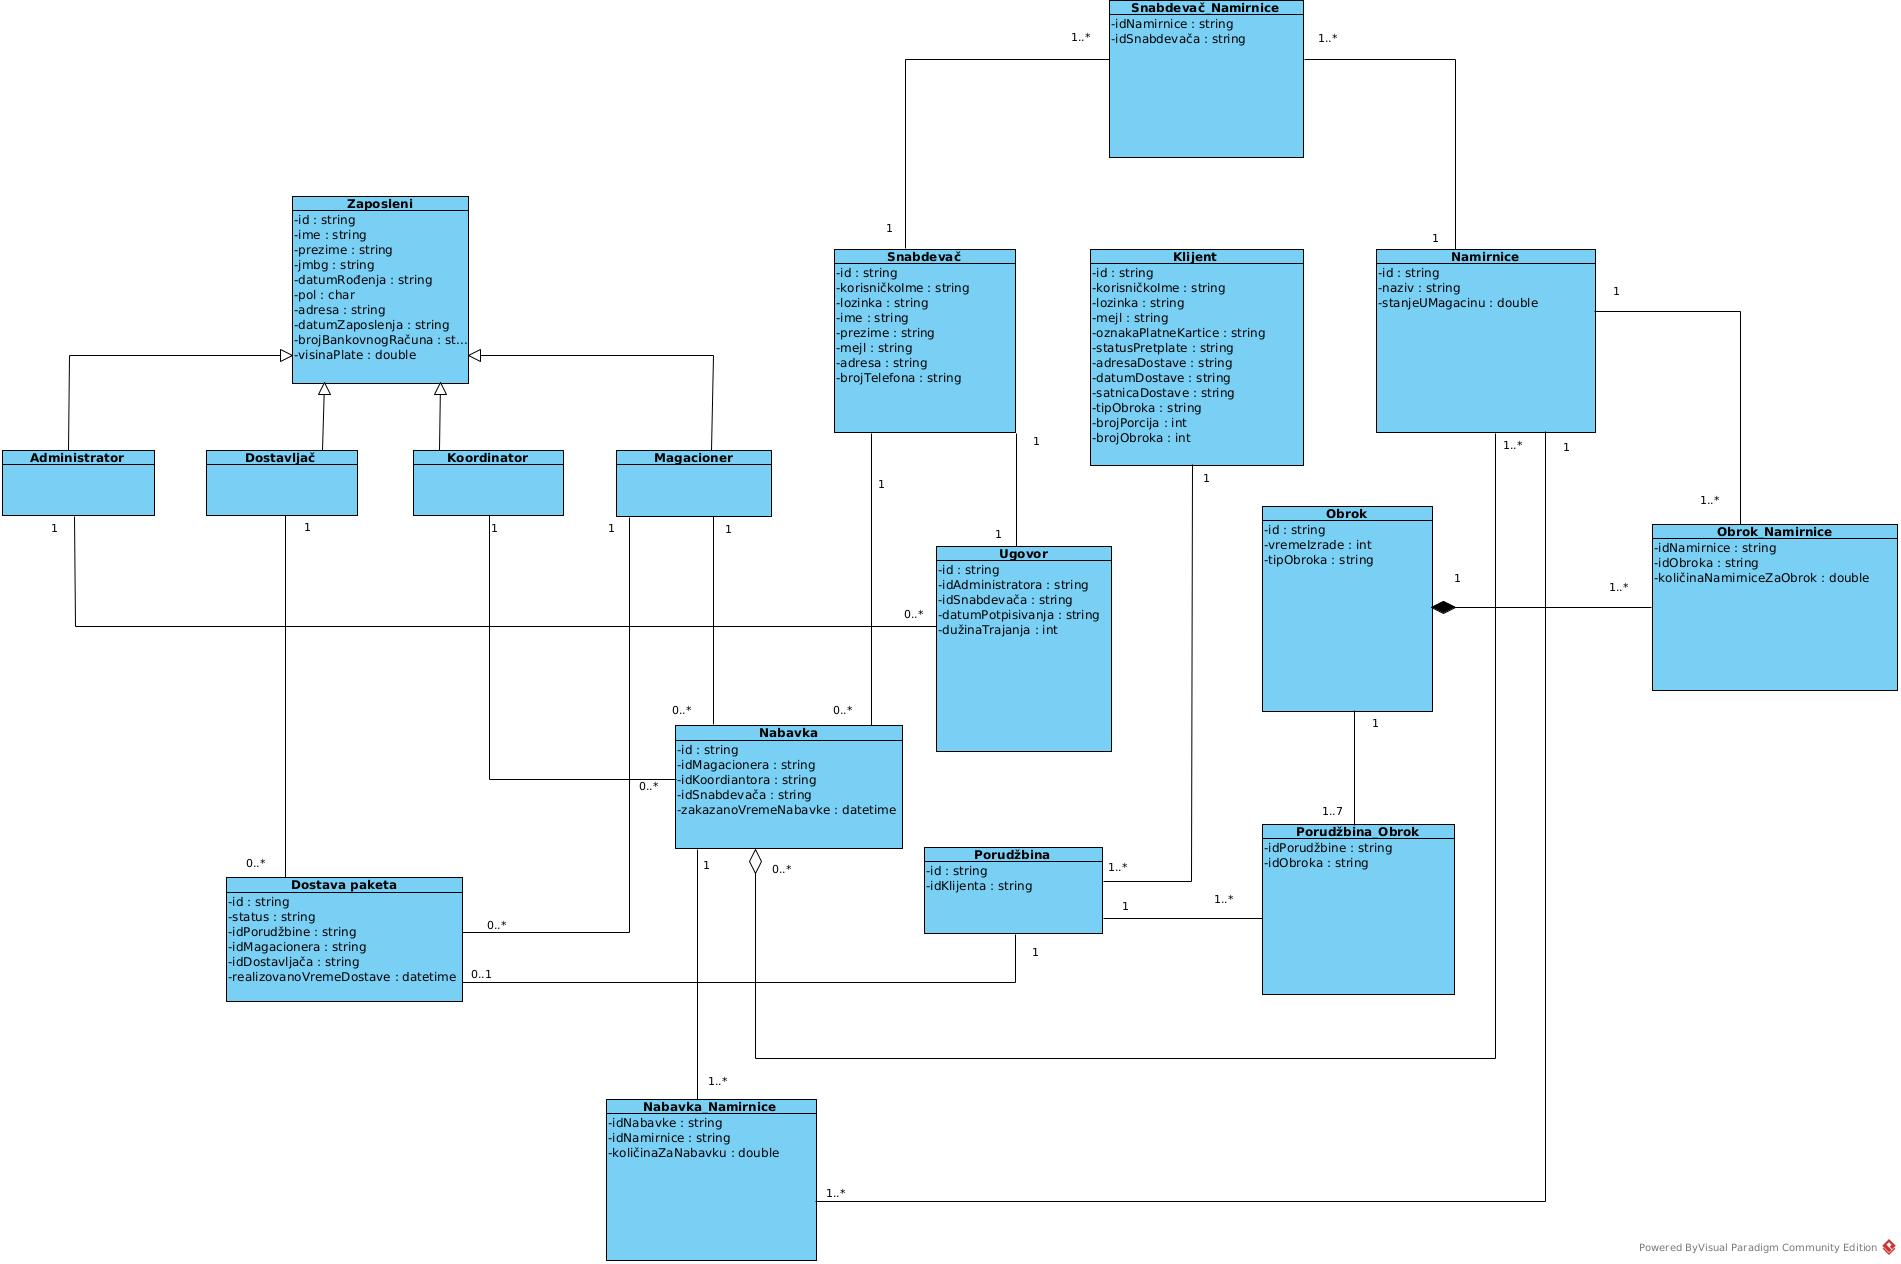
\includegraphics[width=\textwidth]{Pictures/class_diagram_database.jpg}
    		\caption{Dijagram klasa baze podataka}
    \label{fig:ClassDiagramDatabase}
    \end{center}
\end{figure}
